\documentclass[tikz]{standalone}
\begin{document}
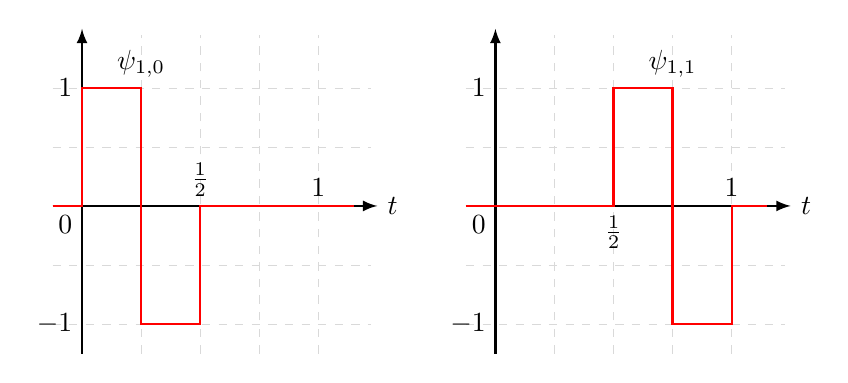
\begin{tikzpicture}[scale=0.75]
  \begin{scope}
  \draw[help lines, color=gray!30, dashed] (-.5,-2.5) grid (4.9,2.9);
  \draw[-latex,thick] (-.5,0)--(5,0) node[right]{$t$};
  \draw[-latex,thick] (0,-2.5)--(0,3);
  \draw[color=red,thick]
      (-.5,0) -- (0,0)
              -- (0,2)
              -- (1,2) node[above,color=black]{$\psi_{1,0}$}
              -- (1,-2)
              -- (2,-2)
              -- (2,0)
              -- (4.6,0);
  \draw
      (0,0) node [anchor=north east] {$0$}
      (0,2) node [left] {$1$}
      (0,-2) node [left] {$-1$}
      (2,0) node [above] {$\frac{1}{2}$}
      (4,0) node [above] {$1$};
  \end{scope}
  \begin{scope}[shift={(7,0)}]
  \draw[help lines, color=gray!30, dashed] (-.5,-2.5) grid (4.9,2.9);
  \draw[-latex,thick] (-.5,0)--(5,0) node[right]{$t$};
  \draw[-latex,thick] (0,-2.5)--(0,3);
  \draw[color=red,thick]
      (-.5,0) -- (2,0)
              -- (2,2)
              -- (3,2) node[above,color=black]{$\psi_{1,1}$}
              -- (3,-2)
              -- (4,-2)
              -- (4,0)
              -- (4.6,0);
  \draw
      (0,0) node [anchor=north east] {$0$}
      (0,2) node [left] {$1$}
      (0,-2) node [left] {$-1$}
      (2,0) node [below] {$\frac{1}{2}$}
      (4,0) node [above] {$1$};
  \end{scope}
\end{tikzpicture}
\end{document}